\documentclass{article}
\usepackage[affil-it]{authblk}
\usepackage{xspace,xcolor}
\usepackage{graphics}
\usepackage[screen,nopanel,white]{pdfscreen}
\hypersetup{pdftoolbar=true}
\usepackage[display]{texpower}

\margins{0.25in}{0.25in}{0.25in}{0.25in}
\screensize{4.5in}{8in}% 4.5in by 8in for widescreen
\backgroundcolor{blue}
\color{white}

\author[1]{Tex Chi}
\author[1]{Jack Li}
\affil[1]{Institute of LaTeX}
\title{pvalueTex}
\begin{document}
\maketitle


\begin{figure}[ht]
%\floatbox[{\capbeside\thisfloatsetup{capbesideposition={right,center},capbesidewidth=.35\linewidth,capbesidesep=quad}}]{figure}[\FBwidth]
%\centering
%\widefigure, keepaspectratio
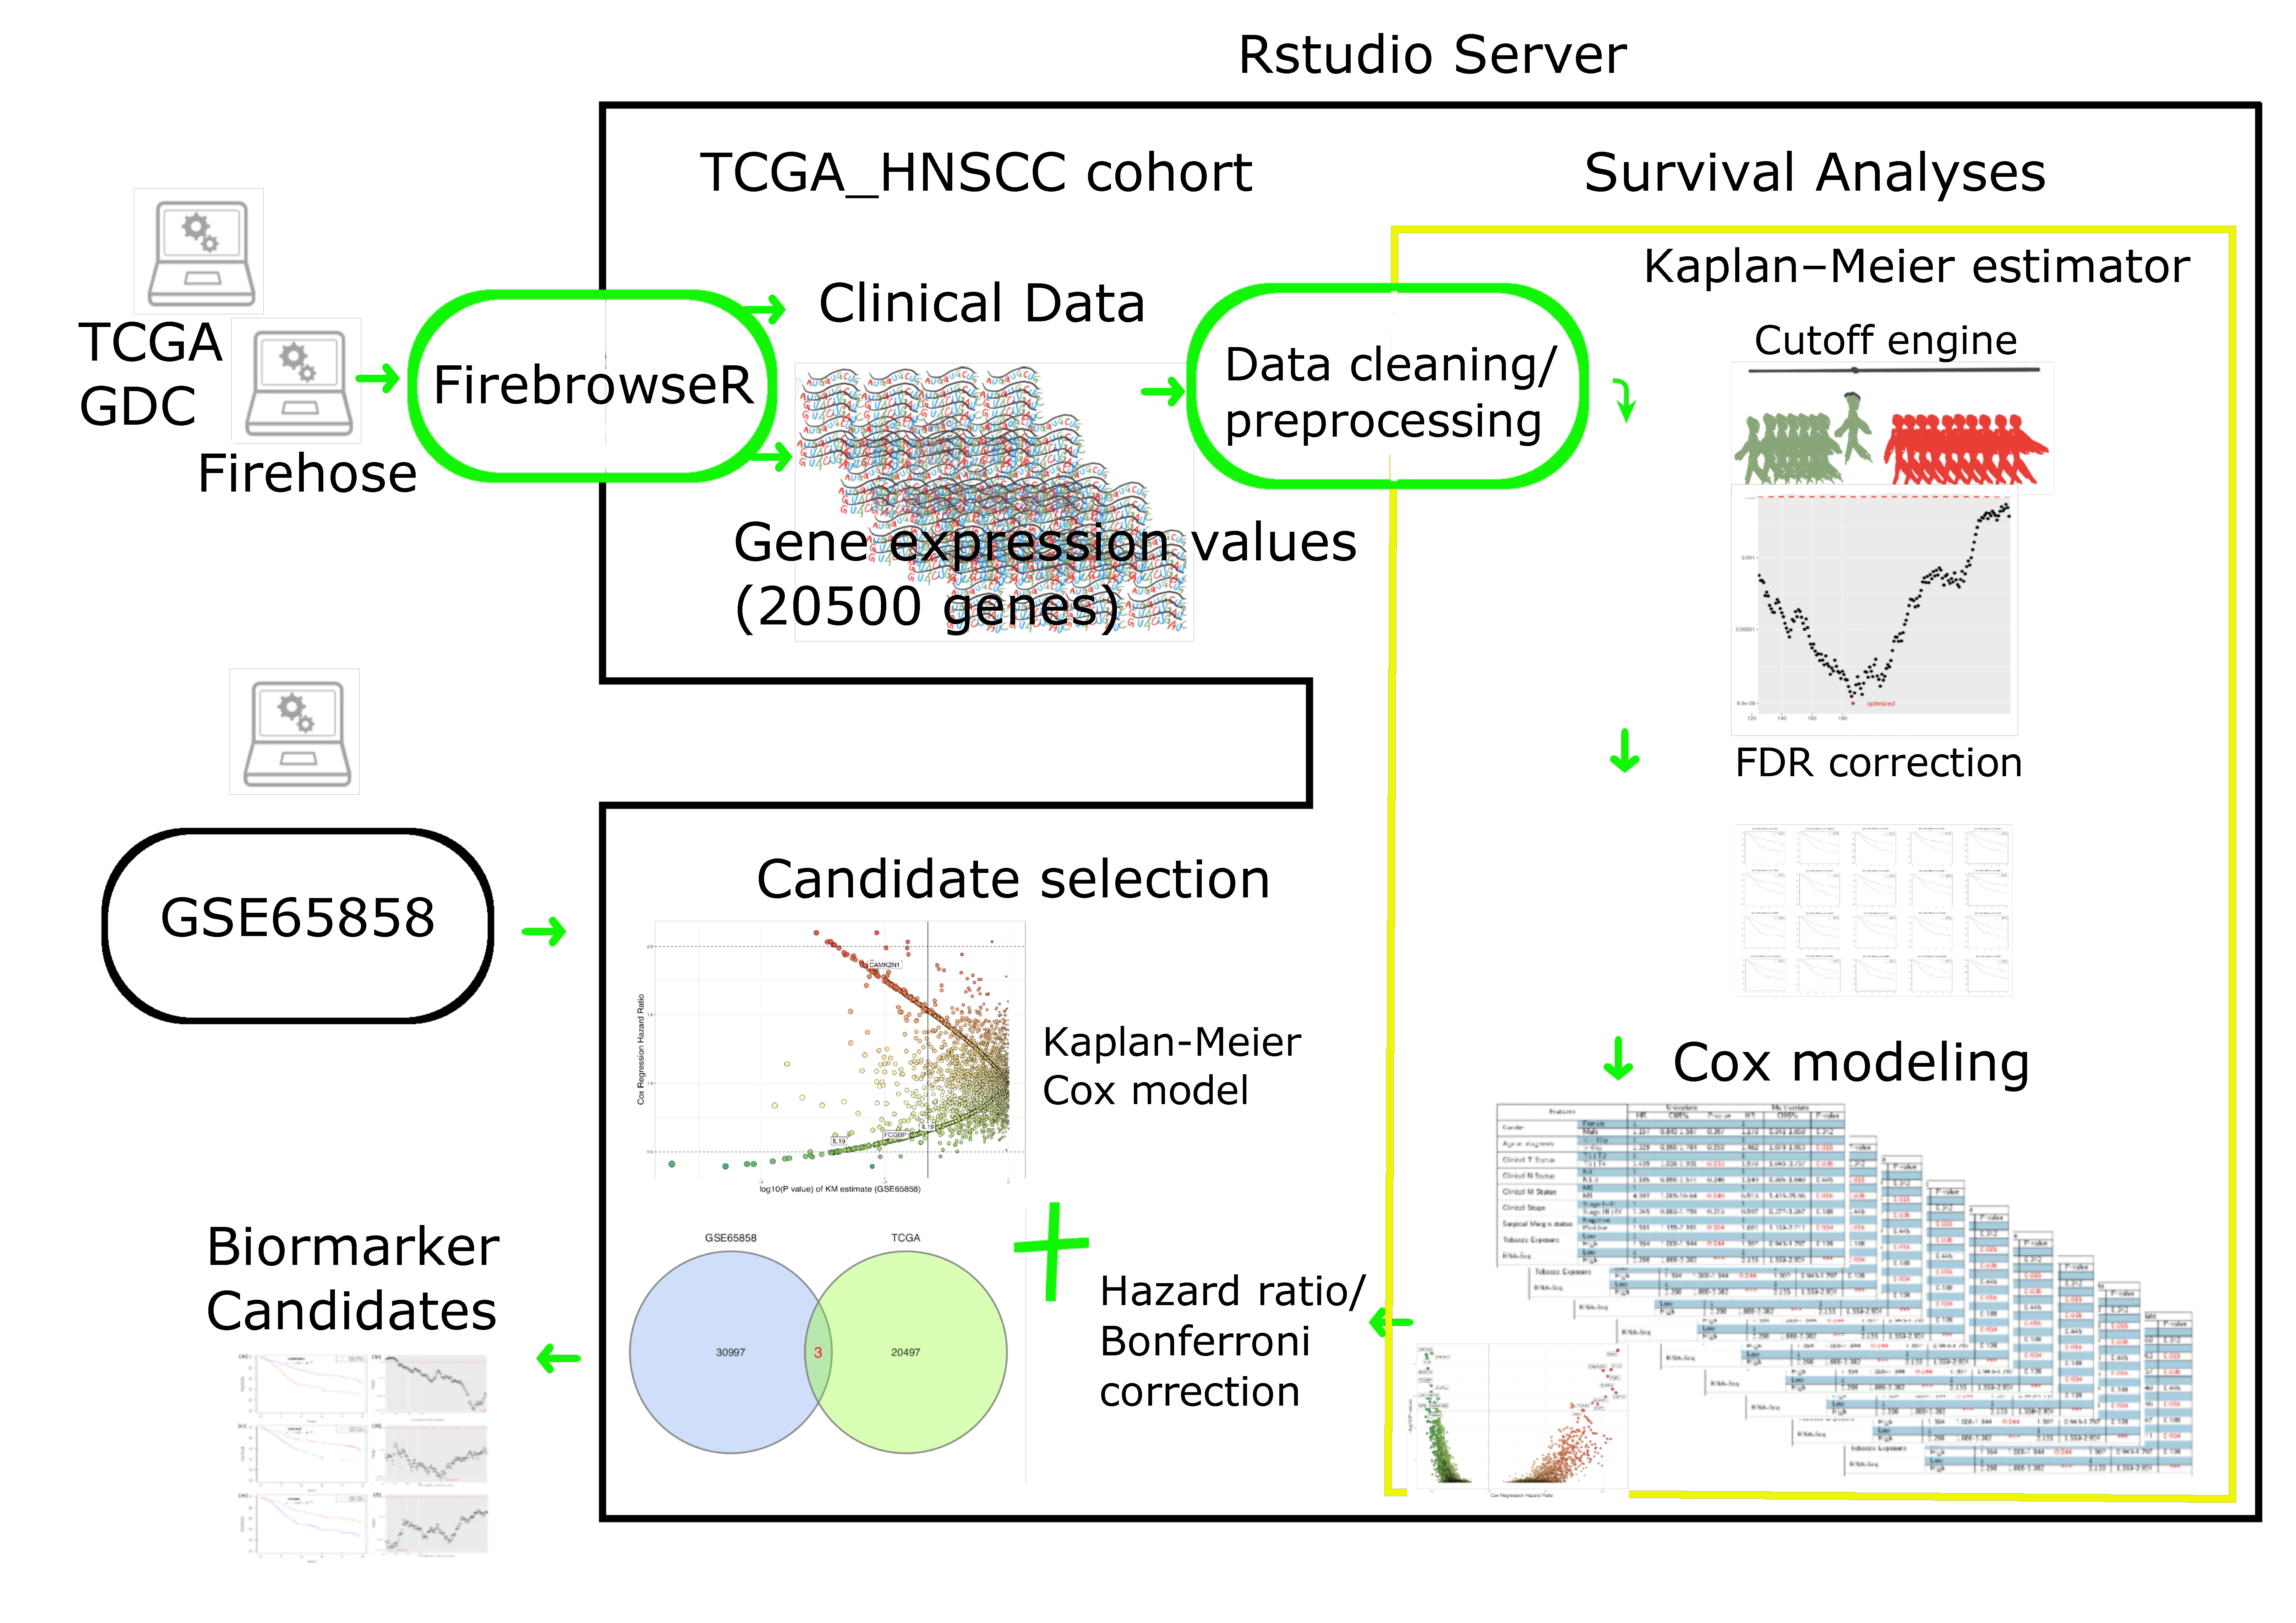
\includegraphics[width=7cm]{Figure_1_manuscript_workflow.pdf} % .PDF is better than .png
%, height=8cm
%\caption % , step 1 (\textcolor{blue}{blue line}: main procedure) and step 2 (\textcolor{orange}{orange line}: analysis export).
%Step 3 (purple line: dealing with surgical margin).
%\sidecaptionvpos{c}
\caption{\hl{A workflow of \acrshort{hnscc} biomarker discovery.\\
The workflow includes data retrieval from the TCGA GDC data portal, data processing with merging and cleaning, and then performing the survival analyses (within \textcolor{yellow}{yellow} square).} The Cutoff engine (in R script: cutofFinder\_func.HNSCC.R, a serial cutoff for grouping patients with \textcolor{asparagus}{low} or \textcolor{red}{high} expression of a specific gene, to yield a collection of \protect\textit{P} values; please see Materials and Methods section for details) might calculate all possible Kaplan--Meier \protect\textit{P} values (corrected by \acrlong{fdr}, FDR, method) to find the optimal cutoff value of gene expression for subsequent Cox modeling. The candidate selection performs (1) dissecting and selection of candidate genes with further Bonferroni adjusted \protect\textit{P} values and the hazard ratios of a Cox model, based on the results from the survival analyses; (2) survival analyses of the other HNSCC dataset (GSE65858) using Kaplan--Meier estimates (with FDR corrections) and Cox modeling.\\ The biomarker candidates were consensus results of TCGA and GSE65858. (HNSCC: head and neck squamous cell carcinoma; TCGA: the Cancer Genome Atlas; RNA-Seq: RNA sequencing; GDC: Genomic Data Commons.)}  % end of caption

% Description:1) FDR correction of Kaplan--Meier \protect\textit{P} values during Cutoff finding; and 2) Bonferroni correction of Kaplan--Meier \protect\textit{P} values after Cox modeling for candidate selection.

%\end{minipage}
\end{figure}

\clearpage

\section{Results}


\section{sec2}
\subsection{sec1.1}

See the data in \ref{fig:1}.

\section*{Figures}
\begin{figure}
    \includegraphics[scale = 0.5]{example-image}
    \caption{No caption, No figure number, No label}
    \label{fig:1}
\end{figure}
\end{document}